\documentclass[11pt, oneside]{article}
\usepackage[letterpaper, margin=2cm]{geometry}
\usepackage{MATH565}

\begin{document}
\noindent \textbf{\Large{Caleb Logemann \\
MATH 565 Continuous Optimization \\
Homework 4
}}

%\lstinputlisting[language=Python]{H01_23.m}
\begin{enumerate}
  \item % #1 Done
    Let $\M{A} \in \RR^{n \times n}$ be a symmetric positive definite matrix.
    \begin{enumerate}
      \item[(a)] % Done
        Show that the unit vectors $\v{d}_1, \v{d}_2, \ldots, \v{d}_n$ are
        $\M{A}$-conjugate vectors if and only if $\M{D}^T \M{A} \M{D} = \M{A}$
        where $\M{D} = \br{\v{d}_1, \v{d}_2, \ldots, \v{d}_n}$.

        \begin{proof}
          First assume that $\set{\v{d}_1, \v{d}_2 \ldots, \v{d}_n}$ are
          $\M{A}$-conjugate.
          Consider the matrix $\M{D} = \br{\v{d}_1, \v{d}_2, \ldots, \v{d}_n}$.
          Then the matrix multiplciation $\M{D}^T \M{A} \M{D}$ results in
          another matrix whose $ij$ entry is $\v{d}_i^T \M{A} \v{d}_j$.
          If $i \neq j$, then $\v{d}_i^T \M{A} \v{d}_j = 0$ because $\v{d}_i$
          and $\v{d}_j$ are $\M{A}$-conjugate.
          If on the other hand $i = j$, then $\v{d}_i^T \M{A} \v{d}_i = 0$
          becuase $\v{d}_i$ is a unit vector with respect to the $\M{A}$-norm.
          This shows that $\M{D}^T \M{A} \M{D} = \M{I}$, because entries on the
          diagonal are $1$ and entries off the diagonal are $0$.

          Now assume that $\M{D}^T \M{A} \M{D} = I$, and consider the set
          $\set{\v{d}_1, \v{d}_2, \ldots, \v{d}_n}$.
          Since $\M{D}^T \M{A} \M{D} = I$, this implies that
          $\v{d}_i^T \M{A} \v{d}_j = 0$ for $i \neq j$ and that
          $\v{d}_i^T \M{A} \v{d}_i = 1$.
          This shows that set $\set{\v{d}_1, \v{d}_2, \ldots, \v{d}_n}$ is
          $\M{A}$-conjugate by definition and that
          $\set{\v{d}_1, \v{d}_2, \ldots, \v{d}_n}$ is normal with respect to
          the $\M{A}$-norm.
        \end{proof}

      \item[(b)] % Done
        If $\M{Q} \in \RR^{n \times n}$ is an orthogonal matrix
        $(\M{Q}^T \M{Q} = \M{I})$, $\v{d}_1, \v{d}_2, \ldots, \v{d_n}$ are
        $\M{A}$-conjugate vectors, and
        $\M{D} = \br{\v{d}_1, \v{d}_2, \ldots, \v{d}_n}$, show that the columns
        of $\M{D} \M{Q}$ are also $\M{A}$-conjugate vectors.

        \begin{proof}
          Consider the matrix product $\p{\M{D} \M{Q}}^T \M{A} \p{\M{D} \M{Q}}$.
          \begin{align*}
            \p{\M{D} \M{Q}}^T \M{A} \p{\M{D} \M{Q}}^T &= \M{Q}^T \M{D}^T \M{A} \M{D} \M{Q}
            \intertext{Since the columns of $\M{D}$ are $\M{A}$-conjugate}
            &= \M{Q}^T I \M{Q} \\
            &= \M{Q}^T \M{Q} \\
            \intertext{Since $\M{Q}$ is orthogonal}
            &= I
          \end{align*}
          This shows by part (a) that the columns of $\M{D} \M{Q}$ are $\M{A}$-
          conjugate.
        \end{proof}
    \end{enumerate}

  \item % #2
    Page 162: Problem 6.3 \\
    Verify that (6.19) and (6.17) are inverses of each other.

  \item % #3 Done
    Page 162: Problem 6.4 \\
    Use the Sherman Morrison formula (A.27) to show that (6.24) is the inverse
    of (6.25).

    \begin{proof}
      The SR1 method has an update method for the matrix $B_k$ given as
      \[
        B_{k+1} = B_k + \frac{(y_k - B_ks_k)(y_k - B_ks_k)^T}{(y_k - B_ks_k)^T s_k}
      \]
      In order to find an update formula for the inverse, $H_{k+1}$ the Sherman-Morrison
      formula can be used, which states that if
      \[
        A_{k+1} = A_k + ab^T
      \]
      then
      \[
        A_{k+1}^{-1} = A_k^{-1} - \frac{A_k^{-1} ab^T A_k^{-1}}{1 + b^T A_k^{-1}a}
      \]
      In our update formula the vectors $a$ and $b$ have the following values.
      \[
        a = \frac{y_k - B_k s_k}{(y_k - B_ks_k)^T s_k}
      \]
      and
      \[
        b = y_k - B_k s_k
      \]

      This means that the update formula for the inverse $H_{k+1}$ can be found
      as follows.
      Note that $H_k$ and $B_k$ are inverses and that $B_k$ and $H_k$ are symmetrical.
      \begin{align*}
        H_{k+1} &= H_k - \frac{1}{(y_k - B_ks_k)^T s_k} \frac{H_k (y_k - B_k s_k)(y_k - B_k s_k)^T H_k}{1 + (y_k - B_k s_k)^T H_k (y_k - B_k s_k)/((y_k - B_ks_k)^T s_k)} \\
        &= H_k - \frac{(H_k y_k - s_k)(y_k^T H_k - s_k^T)}{(y_k - B_ks_k)^T s_k + (y_k - B_k s_k)^T (H_k y_k - s_k)} \\
        &= H_k - \frac{(s_k - H_k y_k)(s_k - H_k y_k)^T}{(y_k^T - s_k^T B_k) s_k + (y_k^T - s_k^T B_k) (H_k y_k - s_k)} \\
        &= H_k - \frac{(s_k - H_k y_k)(s_k - H_k y_k)^T}{y_k^T s_k - s_k^T B_k s_k + y_k^T H_k y_k - y_k^T s_k - s_k^T y_k + s_k^TB_k s_k} \\
        &= H_k - \frac{(s_k - H_k y_k)(s_k - H_k y_k)^T}{y_k^T H_k y_k - y_k^T s_k} \\
        &= H_k - \frac{(s_k - H_k y_k)(s_k - H_k y_k)^T}{(y_k^T H_k - s_k^T) y_k} \\
        &= H_k + \frac{(s_k - H_k y_k)(s_k - H_k y_k)^T}{(s_k^T - y_k^T H_k) y_k} \\
        &= H_k + \frac{(s_k - H_k y_k)(s_k - H_k y_k)^T}{(s_k - H_k y_k)^T y_k} \\
      \end{align*}
      This last update formula is identical to equation (6.25), so this shows
      that (6.24) and (6.25) are indeed inverses of each other.
    \end{proof}

  \item % #4 Done
    Page 162: Problem 6.6 \\
    The square root of a matrix $A$ is a matrix $A^{1/2}$ such that
    $A^{1/2} A^{1/2} = A$.
    Show that symmetric positive definite matrix $A$ has a square root, and that
    this square root is itself symmetric and positive definite.
    % (Hint: Use the factorization A = UDU^T (A.16), where U is orthogonal and D
    % is diagonal with positive diagonal elements)

    \begin{proof}
      Let $A$ be a symmetric positive definite matrix.
      Since $A$ is symmetric positive definite this implies that the
      eigenvalues of $A$ are real and positive and that the eigenvectors of
      $A$ can be chosen to form an orthonormal basis of $\RR^n$.
      This implies that $A$ can be factored as $UDU^T$ where $D$ is a diagonal
      matrix with the eigenvalues of $A$ on the diagonal and where $U$ is an
      orthogonal matrix of the eigenvectors.
      I will define the matrix $D^{1/2}$ as the diagonal matrix whose diagonal
      entries are the positive square roots of the diagonal of $D$.
      This is well-defined as the eigenvalues are strictly greater than zero.
      This can also be shown as
      \begin{align*}
        D &=
        \begin{bmatrix}
          \lambda_1 & & \\
           & \lambda_2 & & \\
           & & \ddots & \\
           & & & \lambda_n
        \end{bmatrix} \\
        D^{1/2} &= 
        \begin{bmatrix}
          \sqrt{\lambda_1} & & \\
           & \sqrt{\lambda_2} & & \\
           & & \ddots & \\
           & & & \sqrt{\lambda_n}
        \end{bmatrix} \\
      \end{align*}
      Note that $D^{1/2} D^{1/2} = D$.
      Now I will define the matrix $A^{1/2} = U D^{1/2} U^T$.
      It can be shown that $A^{1/2} A^{1/2} = A$ since $U^T U = I$ as $U$ is an
      orthogonal matrix.
      \begin{align*}
        A^{1/2} A^{1/2} &= U D^{1/2} U^TU D^{1/2} U^T \\
        &= U D^{1/2} D^{1/2} U^T \\
        &= U D U^T \\
        &= A
      \end{align*}
      Also $A^{1/2}$ is symmetrical as
      \[
        (A^{1/2})^T = (U D^{1/2} U^T)^T = U D^{1/2} U^T = A^{1/2}.
      \]
      Lastly $A^{1/2}$ is positive definite as the eigenvalues of $A^{1/2}$ are
      $\sqrt{\lambda_1}, \sqrt{\lambda_2}, \ldots, \sqrt{\lambda_n}$ which are
      real and positive.

      Thus $A^{1/2}$ satisfies all the criterion for the square root of the
      matrix $A$.
    \end{proof}

  \item % #5 Done
    Implement the BFGS Method (Algorithm 6.1 on Page 140, or lecture notes).

    The following function implements the BFGS Method.
    The input of this function allows the specification of different methods
    for determining alpha.
    \lstinputlisting[language=Matlab]{BFGS.m}

  \item % #6 Done
    Apply the BFGS method to the following function:
    \[
      f(x, y) = (x^2 + y - 11)^2 + (x + y^2 - 7)^2.
    \]
    Use $\M{H}_0 = \M{I}$ and an exact line search for each step length.

    The following script uses the function from \#5.
    \lstinputlisting[language=Matlab]{BFGS.m}

    The function produces the following image, which shows 4 paths converging to the
    four local minima.
    \begin{center}
      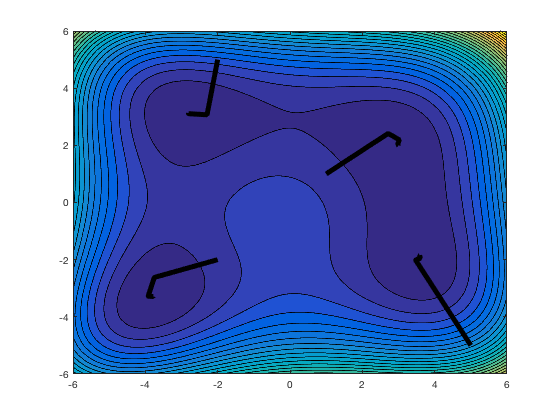
\includegraphics[scale=.7]{Figures/04_1}
    \end{center}

    For all of these paths, I used a tolerance of $10^{-5}$.
    I also used the secant method in order to find the exact $\alpha$ that
    minimized the line search.
    I used the same tolerance for the secant method.

    The first initial point was $(1, 1)$. 
    This path converged to $(3, 2)$ in 7 steps. 
    The value of $f$ at $(3, 2)$ is $f(3, 2) = 0$.

    The second initial point was $(-2, 5)$.
    The BFGS method converged in 5 steps to the point $(-2.8051, 3.1313)$,
    where $f(-2.8051, 3.1313) = 1.0958 \times 10^{-14}$.

    The third initial value was $(-2, -2)$.
    From this initial value the method converged to $(-3.7793, -3.2832)$ in 6
    steps, to a function value of $f(-3.7793, -3.2832) = 2.2437\times e^{-15}$.

    The last initial value was $(5, -5)$.
    This path converged to $(3.5844, -1.8481)$ in 6 steps to a function value
    of $f(3.5844, -1.8481) = 2.0881 \times 10^{-14}$.
\end{enumerate}
\end{document}
